% !TEX encoding = UTF-8
% !TEX TS-program = pdflatex
% !TEX root = ../tesi.tex

%**************************************************************
\chapter{Architettura per computazione parallela}
\label{cap:progettazione-codifica}
%**************************************************************

La precedente architettura risponde all'esigenza di stabilire una comunicazione cross-page, ma lascia irrisolti diversi obiettivi del progetto. In questo capitolo viene invece presentata un'evoluzione di tale architettura, al fine di poter migliorare le performance di \textit{Stargate} ed offrire un sistema di gestione dei widget più indipendente.
Dal punto di vista delle performance, non è difatti sufficiente eseguire le nuove finestre in un processo separato. Sarebbe infatti più ottimale che il calcolo dello \textbf{stato derivato} venga effettuato una volta sola per tutti i widget della stessa tipologia.

\section{Stato derivato}

Per \textit{stato derivato} si intende l'insieme dei dati, calcolati a partire dallo stato applicativo dell'applicazione, necessari al widget per la correttezza esecuzione di tutte le sue funzionalità. La funzione, avente per input lo stato applicativo e per output lo stato derivato, viene convenzionalmente denominata \textbf{selector} ed ha una firma di tipo \texttt{State => DerivedState}.

Tutte le funzioni \textit{selectors} devono inoltre essere pure, ovvero ritornare lo stesso risultato a parità di input e non avere effetti collaterali (\textit{side-effects}), quali accesso/modifica a variabili non locali alla funzione, modifiche per riferimenti, accesso a I/O etc. Maggior informazioni sulle funzioni pure sono reperibili al seguente link: \url{https://en.wikipedia.org/wiki/Pure_function}. \\

Nel seguente esempio lo stato applicativo rappresenta un'applicazione che gestisce una lista di acquisti. Si immagini quindi di avere un widget UI che mostri il totale delle spese e che quindi necessiti di tale stato derivato.

\begin{lstlisting}
interface Purchase {
    name: number
    price: number
}

interface State {
    purchases: Array<Purchase>
}

type DerivedState = number

function sumSelector(state: State): DerivedState {
    let sum: number = 0;

    for (let i = 0; i < state.purchases.length; i++) {
        sum += state.purchases[i].price;
    }

    return sum
}
\end{lstlisting}

Essendo funzioni pure, è possibile comporre \textit{selectors} nella stessa maniera in cui si compongono funzioni matematica \texttt{f . g}, ottenendo \textit{selectors} più complessi ma comunque modulari. Il \textit{selector} finale di un componente UI può essere il risultato di decine di sotto-selectors, a loro volte composti da altri selectors.

\begin{figure}[H] 
  \centering 
  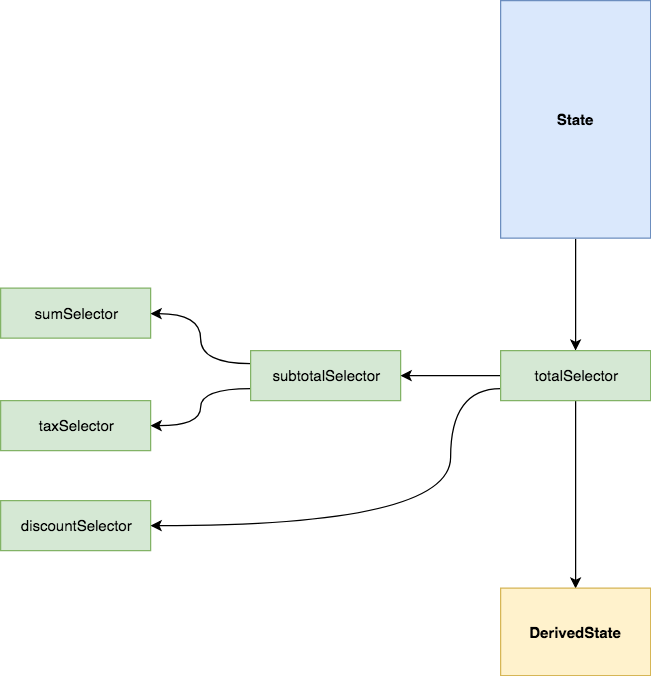
\includegraphics[width=1\columnwidth]{selectors} 
  \caption{Esempio di composizione di selectors}
\end{figure}

È facile quindi immaginare che in un componente UI complesso quale una mappa dei veicoli e rotte, tali \textit{selectors} siano molto complessi e richiedano un tempo di computazione non indifferente. \\

In particolare il codice JavaScript dell'applicazione principale è eseguito in un unico thread, per cui calcolare nell'applicazione padre lo stato derivato di diverse finestre con mappe potrebbe bloccare l'applicazione e renderla incapace di rispondere alle interazioni utenti fino al termine dei calcoli nei \textit{selectors}. 

Una possibile soluzione potrebbe essere delegare tale calcolo nelle finestre figlie, poiché vivono su processi dedicati. Sebbene sia accettabile, non è ottimale in quanto il calcolo dei \textit{selectors} è ripetuto anche se è identico per due finestre aventi entrambe la stessa tipologia di widget, per cui esiste un'alternativa migliore.

L'ideale è difatti calcolare lo stato derivato per ciascun tipo di widget, ad esempio per tutte le finestre contenenti la mappa, una sola volta ad ogni modifica dello stato applicativo e propagare il risultato del calcolo ai widget. In tal modo l'onere computazionale è linearmente dipendente dal numero di \textbf{tipi di widget} attivi invece che dal numero totale di widget. Tuttavia tale calcolo allo stesso tempo non può avere nella finestra padre per le ragioni descritte sopra.


